\documentclass[10pt,a4paper]{article}
\usepackage[utf8]{inputenc}
\usepackage{pgfplots}
\pgfplotsset{compat=1.16}
\usepackage{tikz}
\usetikzlibrary{automata,topaths,arrows,shapes}
\usetikzlibrary{backgrounds}
\usepackage{xcolor}
\usepackage{amsmath}
\usepackage{amssymb}

\begin{document}

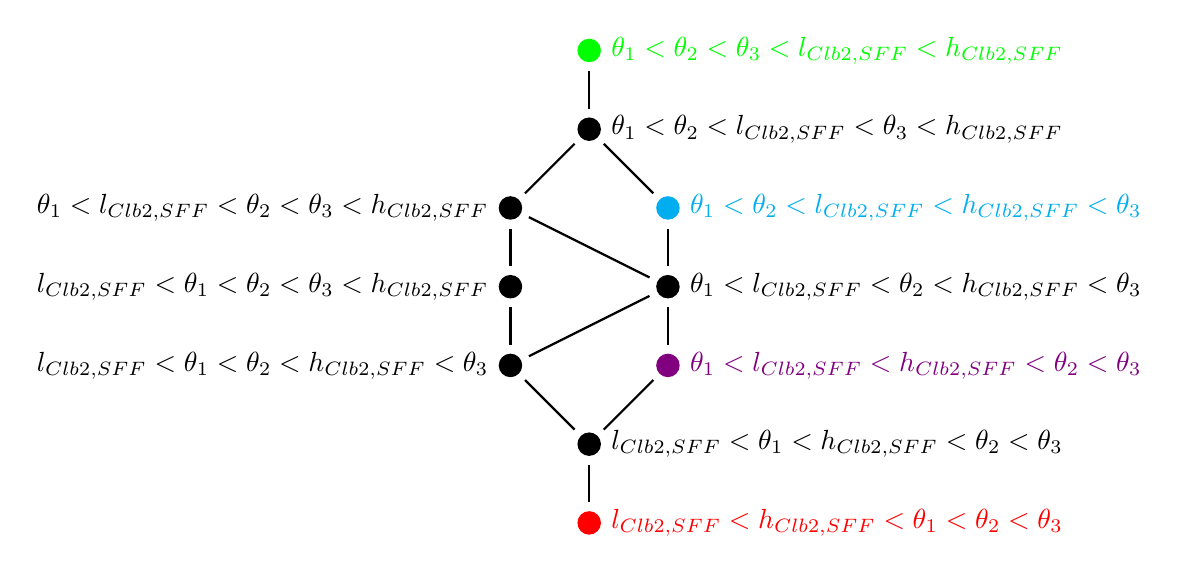
\begin{tikzpicture}
\node (n1) at (0,5) [label=left:$\theta_1<l_{Clb2,SFF}<\theta_2<\theta_3<h_{Clb2,SFF}$,circle,fill,inner sep=3pt]{};
\node (n2) at (0,4)[label=left:$l_{Clb2,SFF}<\theta_1<\theta_2<\theta_3<h_{Clb2,SFF}$,circle,fill,inner sep=3pt]{};
\node (n3) at (0,3) [label=left:$l_{Clb2,SFF}<\theta_1<\theta_2<h_{Clb2,SFF}<\theta_3$,circle,fill,inner sep=3pt]{};
\node[color=green] (n4) at (1,7)[label=right:\textcolor{green}{$\theta_1<\theta_2<\theta_3<l_{Clb2,SFF}<h_{Clb2,SFF}$},circle,fill,inner sep=3pt]{};
\node (n5) at (1,6) [label=right:$\theta_1<\theta_2<l_{Clb2,SFF}<\theta_3<h_{Clb2,SFF}$,circle,fill,inner sep=3pt]{};
\node[color=cyan] (n6) at (2,5)[label=right:\textcolor{cyan}{$\theta_1<\theta_2<l_{Clb2,SFF}<h_{Clb2,SFF}<\theta_3$},circle,fill,inner sep=3pt]{};
\node (n7) at (2,4) [label=right:$\theta_1<l_{Clb2,SFF}<\theta_2<h_{Clb2,SFF}<\theta_3$,circle,fill,inner sep=3pt]{};
\node[color=violet] (n8) at (2,3)[label=right:\textcolor{violet}{$\theta_1<l_{Clb2,SFF}<h_{Clb2,SFF}<\theta_2<\theta_3$},circle,fill,inner sep=3pt]{};
\node (n9) at (1,2) [label=right:$l_{Clb2,SFF}<\theta_1<h_{Clb2,SFF}<\theta_2<\theta_3$,circle,fill,inner sep=3pt]{};
\node[color=red] (n10) at (1,1)[label=right:\textcolor{red}{$l_{Clb2,SFF}<h_{Clb2,SFF}<\theta_1<\theta_2<\theta_3$},circle,fill,inner sep=3pt]{};



\path[>=angle 90,thick]
(n1) edge[shorten <= 3pt, shorten >= 3pt] node[] {} (n2)
(n2) edge[shorten <= 3pt, shorten >= 3pt,] node[] {} (n3)
(n3) edge[shorten <= 3pt, shorten >= 3pt] node[] {} (n9)
(n1) edge[shorten <= 3pt, shorten >= 3pt] node[] {} (n7)
(n3) edge[shorten <= 3pt, shorten >= 3pt] node[] {} (n7)
(n5) edge[shorten <= 3pt, shorten >= 3pt] node[] {} (n1)
(n4) edge[ shorten <= 3pt, shorten >= 3pt] node[] {} (n5)
(n5) edge[shorten <= 3pt, shorten >= 3pt] node[] {} (n6)
(n6) edge[shorten <= 3pt, shorten >= 3pt] node[] {} (n7)
(n7) edge[shorten <= 3pt, shorten >= 3pt] node[] {} (n8)
(n8) edge[ shorten <= 3pt, shorten >= 3pt] node[] {} (n9)
(n9) edge[shorten <= 3pt, shorten >= 3pt] node[] {} (n10)

;                       
\end{tikzpicture}

\end{document}